%----------------------------------------------------------------------------------------
%    PACKAGES AND THEMES
%----------------------------------------------------------------------------------------

\documentclass[aspectratio=169,xcolor=dvipsnames]{beamer}
\setbeameroption{show notes} %TODO: Thomas a enlever avant la presentation
\usetheme{SimplePlus}

\usepackage{comment}
\usepackage{hyperref}
\usepackage{graphicx} % Allows including images
\usepackage{booktabs} % Allows the use of \toprule, \midrule and \bottomrule in tables
\usepackage{array} % Allows >{\centering\arraybackslash} in tabular

%----------------------------------------------------------------------------------------
%    TITLE PAGE
%----------------------------------------------------------------------------------------

\title{Stochastic Optimal Control Matching}
\subtitle{Carles Domingo-Enrich, Jiequn Han, Brandon Amos, Joan Bruna, Ricky T. Q. Chen}

\author{Thomas Mousseau}

% \institute
% {
%     Department of Computer Science and Information Engineering \\
%     National Taiwan University % Your institution for the title page
% }
\date{\today} % Date, can be changed to a custom date

%----------------------------------------------------------------------------------------
%    PRESENTATION SLIDES
%----------------------------------------------------------------------------------------

\begin{document}

\begin{frame}
    % Print the title page as the first slide
    \titlepage
\end{frame}

\begin{frame}{Overview}
    % Throughout your presentation, if you choose to use \section{} and \subsection{} commands, these will automatically be printed on this slide as an overview of your presentation
    \tableofcontents
\end{frame}

%------------------------------------------------
\section{Setup and Preliminaries}

\begin{frame}{Generative Models}
    \begin{center}
        \begin{minipage}{0.9\textwidth}

            \begin{block}{The Core Challenge: Unnormalized Densities}
                Generative models must sample from complex distributions $p_{\text{data}}(x) = \frac{1}{Z} \tilde{p}_{\text{data}}(x)$ where the normalization constant $Z = \int \tilde{p}_{\text{data}}(x) dx$ is intractable to compute. This intractability arises from the curse of dimensionality when integrating over high-dimensional spaces.
            \end{block}

            \vspace{0.3cm}

            \begin{tabular}{@{}l@{\hspace{0.8cm}}p{0.85\textwidth}@{}}
                \textbf{2020} & \textbf{DDPM:} Denoising Diffusion Probabilistic Models interpret generation as reversing a discrete noise-adding process, learning to denoise at each step. They produced high-quality samples but required thousands of slow sampling steps. \\[0.2cm]
                
                % \textbf{2021} & \textbf{Score-based Models:} Score-based generative models extended diffusion to continuous-time SDEs, learning the score function ($\nabla_x \log p_t(x)$) to reverse a stochastic diffusion process. This unified diffusion with stochastic control, allowed probability flow ODEs, and sped up sampling. \\[0.4cm]
                
                \textbf{2023} & \textbf{Flow Matching:} Flow matching views generation as learning a deterministic ODE vector field that directly transports a simple distribution (e.g., Gaussian) to data. This removed stochasticity and significantly improved efficiency compared to diffusion/score methods. \\[0.2cm]
            \end{tabular}
            
            \vspace{0.3cm}
        \end{minipage}
    \end{center}
\end{frame}

\begin{frame}{SOC as the Foundation of Generative Models}
    \vspace{-0.3cm}
    % \begin{block}{The Core Challenge: Unnormalized Densities}
    %     Generative models must sample from complex distributions $p_{\text{data}}(x) = \frac{1}{Z} \tilde{p}_{\text{data}}(x)$ where the normalization constant $Z = \int \tilde{p}_{\text{data}}(x) dx$ is intractable to compute. This intractability arises from the curse of dimensionality when integrating over high-dimensional spaces.
    % \end{block}

    % \vspace{-0.3cm}

        \begin{alertblock}{SOC Connection}
            Transform tractable distributions (Gaussian) to complex target distributions through \textcolor{blue}{optimal control policies}.
            
            \vspace{0.3cm}
            
            This bridges the gap between:
            \begin{itemize}
                \item Simple sampling (easy)
                \item Complex data distributions (hard)
            \end{itemize}

            From Langevin dynamics to modern diffusion models, all major breakthroughs in generative modeling can be understood through the lens of stochastic optimal control theory.

        \end{alertblock}
        
    % \note{
    % \textcolor{blue}{\textbf{Unnormalized Densities:}} The fundamental challenge in generative modeling is sampling from distributions $p(x) = \frac{1}{Z}e^{-E(x)}$ where $Z$ is unknown. SOC provides the mathematical framework to construct sampling procedures. \\
    % \vspace{0.1cm}
    % \textcolor{orange}{\textbf{Historical Context:}} From Langevin dynamics to modern diffusion models, all major breakthroughs in generative modeling can be understood through the lens of stochastic optimal control theory.
    % }
\end{frame}

\begin{frame}{What is a Stochastic Control Problem?}
    
    \begin{block}{Control-Affine Stochastic Differential Equation}
        The general form of a controlled stochastic process:
        \begin{equation}
        dX_t^u = \big(b(X_t^u, t) + \sigma(t)u(X_t^u, t)\big) dt + \sqrt{\lambda}\sigma(t) dB_t
        \end{equation}
    \end{block}

            \vspace{0.3cm}
    
            \textbf{State Process:} $X_t^u \in \mathbb{R}^d$ (system state under control $u$ at time $t$)
            
            \vspace{0.3cm}
            
            \textbf{Drift Term:} $b(X_t^u, t) \in \mathbb{R}^d$ (natural evolution of the system)
            
            \vspace{0.3cm}
            
            \textbf{Control Term:} $u(X_t^u, t) \in \mathbb{R}^d$ (how control influences the system)
            
            \vspace{0.3cm}
            
            \textbf{Diffusion Coefficient:} $\sigma(t) \in \mathbb{R}^{d \times d}$ (volatility matrix)
            
            \vspace{0.3cm}
            
            \textbf{Noise Process:} $B_t \in \mathbb{R}^d$ (Brownian motion, external randomness)
            
            \vspace{0.3cm}
            
            \textbf{Noise Intensity:} $\lambda > 0$ (controls the strength of stochastic perturbations)

%     \note{
%     \textcolor{blue}{\textbf{Control-Affine Structure:}} The "control-affine" property means the control $u$ enters linearly (affinely) in the drift term. This is the most general practical form for controlled SDEs, encompassing most applications in finance, robotics, and machine learning. \\    
%     \vspace{0.1cm}

%    \textcolor{red}{Je dois aussi expliquer l'importance que le steering input ainsi que le noise sont tous les 2 multipliés par sigma(t) ce qui signifie que ...}
%     }
\end{frame}

\begin{frame}{The Optimal Control Objective}
    \vspace{-0.3cm}
    
    \begin{block}{Cost Function to Minimize}
        Find the optimal control policy $u^* \in \mathcal{U}$ that minimizes:
        \begin{equation}
        \min_{u \in \mathcal{U}} \mathbb{E}\left[\int_0^T \left(\frac{1}{2}\|u(X_t^u, t)\|^2 + f(X_t^u, t)\right) dt + g(X_T^u)\right]
        \end{equation}
    \end{block}

            \vspace{0.3cm}
    
             \textbf{Control Effort:} $\frac{1}{2}\|u(X_t^u, t)\|^2$ (penalizes large control actions)

            \vspace{0.3cm}

             \textbf{Running Cost:} $f(X_t^u, t)$ (ongoing cost during the process evolution)

            \vspace{0.3cm}

             \textbf{Terminal Cost:} $g(X_T^u)$ (final cost based on end state at time $T$)
            
            \vspace{0.3cm}
            
             \textbf{Control Space:} $\mathcal{U}$ (set of admissible control policies)

    % \note{

    % }
    
\end{frame}

\begin{frame}{SOC in Practice}

    \vspace{-0.3cm}
    \begin{table}
        \centering
        \small
        \begin{tabular}{>{\centering\arraybackslash}p{0.25\textwidth}|>{\centering\arraybackslash}p{0.22\textwidth}|>{\centering\arraybackslash}p{0.22\textwidth}|>{\centering\arraybackslash}p{0.22\textwidth}}
            \toprule
            \textbf{Aspect} & \textbf{Steering Actuator} & \textbf{Diffusion Models} & \textbf{Flow Models} \\
            \midrule
            \textbf{State $X_t$} & Vehicle position, velocity & Noisy data sample & Clean data sample \\
            \midrule
            \textbf{Control $u_t$} & Steering angle, throttle & Denoising direction & Flow velocity field \\
            \midrule
            \textbf{Dynamics Source} & \textcolor{blue}{Newtonian mechanics} & \textcolor{orange}{Forward noising process} & \textcolor{ForestGreen}{No natural drift} (learnable) \\
            \midrule
            \textbf{Drift $b(X_t,t)$} & Vehicle dynamics & Predetermined schedule & $b = 0$ (control learns drift) \\
            \midrule
            \textbf{Control Goal} & Reach target safely & Reverse noise process & Transport distributions \\
            \midrule
            \textbf{Noise $\sqrt{\lambda}\sigma dB_t$} & Road disturbances & Brownian motion & Optional stochasticity \\
            \bottomrule
        \end{tabular}
    \end{table}
    
    \vspace{0.3cm}
    
    \begin{alertblock}{Key Insight}
        \textbf{Same mathematical framework, different physics:} SOC unifies vehicle control, generative modeling, and distribution transport under a single theoretical umbrella.
    \end{alertblock}

    % \note{
    % \textcolor{blue}{\textbf{Steering Actuator:}} The dynamics come from well-established physics - Newton's laws, kinematics, and vehicle dynamics. The control optimizes safety and efficiency. \\
    % \vspace{0.1cm}
    % \textcolor{orange}{\textbf{Diffusion Models:}} The drift is determined by the forward noising process (e.g., $\beta(t)$), and control learns to reverse this predetermined corruption. \\
    % \vspace{0.1cm}
    % \textcolor{ForestGreen}{\textbf{Flow Models:}} No natural drift exists - the control $u_t$ directly becomes the drift term, learning the entire velocity field that transports distributions.
    % }
\end{frame}

%------------------------------------------------
\section{Stochastic Optimal Control Matching}

\begin{frame}{Applications of SOC}
    
    \begin{block}{Key ML Applications of SOC}
        \begin{itemize}
            \item \textbf{Reward fine-tuning of diffusion and flow models:} Optimizing generation quality using reward signals
            
            \vspace{0.2cm}
            
            \item \textbf{Conditional sampling on diffusion and flow models:} Steering generation towards specific conditions or constraints
            
            \vspace{0.2cm}
            
            \item \textbf{Sampling from unnormalized densities:} Efficiently drawing samples from complex, intractable distributions
            
            \vspace{0.2cm}
            
            \item \textbf{Importance sampling of rare events in SDEs:} Computing probabilities of low-probability but critical events
        \end{itemize}
    \end{block}

    \vspace{-0.1cm}
    
    \begin{alertblock}{Key Insight}
        The prevalence of SOC formulations in modern ML motivates the need for more efficient and stable solving methods.
    \end{alertblock}

    % \note{\textcolor{red}{Je dois etre capable de vraiment bien expliquer les applications du SOC dans le ML moderne pour pouvoir demontrer l'importance d'avoir pris ce papier}}
\end{frame}

\begin{frame}{Solve SOC Problems in Low Dimension}
    \vspace{-0.1cm}
    
    \begin{block}{Classical Approach: Hamilton-Jacobi-Bellman PDE}
        In small state spaces, discretize the state space and solve the HJB PDE directly. After applying dynamic programming and Bellman's optimality principle we get:
        \begin{equation}
        \frac{\partial V}{\partial t} + \min_u \left[ \frac{1}{2}\|u\|^2 + f(x,t) + \nabla V \cdot (b + \sigma u) + \frac{1}{2}\lambda \text{tr}(\sigma^T \nabla^2 V \sigma) \right] = 0
        \end{equation}
    \end{block}

    \vspace{-0.4cm}
    
    \begin{columns}[t]
        \column{0.48\textwidth}
        \begin{block}{What You Get}
            \begin{itemize}
                \item \textcolor{ForestGreen}{\textbf{Value function:}} $V(x,t)$
                \item \textcolor{ForestGreen}{\textbf{Optimal control:}} $u^*(x,t) = -\sigma(t)^T \nabla V(x,t)$
                \item \textcolor{ForestGreen}{\textbf{Global optimum}} guaranteed
                \item \textcolor{ForestGreen}{\textbf{Theoretical guarantees}} (convergence, stability)
            \end{itemize}
        \end{block}
        
        \column{0.48\textwidth}
        \begin{alertblock}{The Curse of Dimensionality}
            \begin{itemize}
                \item \textcolor{red}{\textbf{Grid size:}} $\mathcal{O}(N^d)$ where $d$ is dimension
                \item \textcolor{red}{\textbf{Memory:}} Exponential growth with $d$
                \item \textcolor{red}{\textbf{Computation:}} Infeasible for $d > 3$
            \end{itemize}
        \end{alertblock}
    \end{columns}
    % \note{
    %     \textbf{Works perfectly in low dimensions, but state space grows exponentially with dimension.}

    % \textcolor{blue}{\textbf{Classical HJB:}} In low dimensions, you can discretize the entire state space on a grid and solve the HJB PDE using finite difference methods. This gives you the exact solution but becomes computationally impossible as dimension increases. \\
    % \vspace{0.1cm}
    % \textcolor{red}{\textbf{Curse of Dimensionality:}} For a $d$-dimensional problem with $N$ grid points per dimension, you need $N^d$ total grid points. Even modest problems ($d=10$, $N=100$) require $100^{10} = 10^{20}$ grid points.
    % }
\end{frame}

\begin{frame}{Solve SOC Problems in High Dimension}
    \vspace{-0.1cm}
    
    \begin{block}{Modern Approach: Adjoint Methods}
        Cannot discretize high-dimensional spaces, so use \textcolor{blue}{\textbf{adjoint methods}} to optimize control directly:
        \begin{equation}
        \min_{u} \mathbb{E}\left[\int_0^T \left(\frac{1}{2}\|u(X_t^u, t)\|^2 + f(X_t^u, t)\right) dt + g(X_T^u)\right]
        \end{equation}
    \end{block}

    \vspace{-0.4cm}

    \begin{columns}[t]
        \column{0.48\textwidth}
        \begin{block}{What You Get}
            \begin{itemize}
                \item \textcolor{ForestGreen}{\textbf{Scalable:}} Works in high dimensions
                \item \textcolor{ForestGreen}{\textbf{Neural networks:}} Can parameterize complex controls
                \item \textcolor{ForestGreen}{\textbf{Gradient-based:}} Standard optimization techniques
            \end{itemize}
        \end{block}
        
        \column{0.48\textwidth}
        \begin{alertblock}{Major Problem}
            \begin{itemize}
                \item \textcolor{red}{\textbf{Non-convex landscape:}} Full of local minima
                \item \textcolor{red}{\textbf{Unstable training:}} Difficult optimization
                \item \textcolor{red}{\textbf{No guarantees:}} May not find global optimum
            \end{itemize}
        \end{alertblock}
    \end{columns}
\end{frame}

\begin{frame}{Similar Trend in Generative Modeling}
    \vspace{-0.1cm}
    
    \begin{block}{The Same Pattern: Non-convex → Least-Squares}
        Generative modeling experienced the same transition from non-convex to convex optimization
    \end{block}
        
    \vspace{-0.4cm}

    \begin{columns}[t]
        \column{0.48\textwidth}
        \begin{alertblock}{Continuous Normalizing Flows}
            \small
            \textbf{Method:} Learn invertible transformations
            \begin{equation}
            \frac{dx}{dt} = f_\theta(x, t)
            \end{equation}
            
            \textbf{Problem:}
            \begin{itemize}
                \item Use \textcolor{red}{\textbf{adjoint methods}} for gradients
                \item \textcolor{red}{\textbf{Non-convex}} optimization landscape
                \item Difficult training, unstable dynamics
            \end{itemize}
        \end{alertblock}
        
        \column{0.48\textwidth}
        \begin{block}{Denoising Diffusion Models}
            \small
            \textbf{Method:} Learn to reverse noise process
            \begin{equation}
            \mathbb{E}[\|\epsilon_\theta(x_t, t) - \epsilon\|^2]
            \end{equation}
            
            \textbf{Advantage:}
            \begin{itemize}
                \item Use \textcolor{ForestGreen}{\textbf{least-squares loss}} 
                \item \textcolor{ForestGreen}{\textbf{Convex}} functional landscape
                \item Stable, reliable optimization
            \end{itemize}
        \end{block}
    \end{columns}
        
    % \note{
    % \textbf{Insight:} Apply the same principle to SOC! Replace non-convex adjoint methods with \textcolor{blue}{\textbf{least-squares matching}}, creating a \textcolor{ForestGreen}{\textbf{convex optimization landscape}} for stochastic optimal control.
    % \\
    % \vspace{0.1cm}
    % \textcolor{orange}{\textbf{Historical Parallel:}} Continuous Normalizing Flows (CNFs) suffered from the same optimization challenges as traditional SOC - they used adjoint methods and had non-convex landscapes. DDPMs revolutionized generative modeling by reformulating the problem as least-squares regression. \\
    % \vspace{0.1cm}
    % \textcolor{blue}{\textbf{SOCM's Contribution:}} SOCM brings the same insight to stochastic optimal control, replacing direct optimization with least-squares matching to achieve stable, convex optimization.
    % }
\end{frame}


\begin{frame}{Optimization Landscapes}
    \vspace{0.5cm}
    \begin{table}
        \centering
        \begin{tabular}{>{\centering\arraybackslash}p{0.25\textwidth}>{\centering\arraybackslash}p{0.35\textwidth}>{\centering\arraybackslash}p{0.35\textwidth}}
            \toprule
            \textbf{Task} & \textbf{Non-convex} & \textbf{Least Squares} \\
            \midrule
            Generative Modeling & Maximum Likelihood CNFs & Diffusion models and Flow Matching \\
            Stochastic Optimal Control & Adjoint Methods & \textcolor{red}{\textbf{Stochastic Optimal Control Matching}} \\
            \bottomrule
        \end{tabular}
    \end{table}
\end{frame}

\begin{frame}{From Classical SOC to SOCM}
    \small
    \begin{block}{Dynamics (Same for Both)}
        \begin{equation}
        dX^v_t = (b(X^v_t, t) + \sigma(t)v(X^v_t, t)) dt + \sqrt{\lambda}\sigma(t) dB_t \text{, with } X^v_0 \sim p_0
        \end{equation}
    \end{block}

    \begin{block}{Original SOC Cost Function}
        \begin{equation}
        \min_{u \in \mathcal{U}} \mathcal{L}_{SOC} := \mathbb{E}\left[\int_0^T \left(\frac{1}{2}\|u(X_t^u, t)\|^2 + f(X_t^u, t)\right) dt + g(X_T^u)\right]
        \end{equation}
    \end{block}

    \begin{alertblock}{SOCM Cost Function}
        \begin{equation}
        \min_{u, M} \mathcal{L}_{SOCM}(u, M) := \mathbb{E}\left[\frac{1}{T}\int_0^T \|u(X^v_t, t) - w(t, v, X^v, B, M_t)\|^2 dt \times \alpha(v, X^v, B)\right]
        \end{equation}
    \end{alertblock}

    \vspace{0.2cm}
    \small
    \textbf{Key Point:} Same underlying stochastic dynamics, but SOCM uses a \textcolor{blue}{least-squares matching approach} instead of direct minimization of the original cost.
\end{frame}

\begin{frame}{SOCM Parameters Definition}
    
    $$\min_{\textcolor{blue}{u}, \textcolor{red}{M}} \mathcal{L}_{SOCM}(\textcolor{blue}{u}, \textcolor{red}{M}) := \mathbb{E}\left[\frac{1}{T}\int_0^T \|\textcolor{blue}{u}(X^{\textcolor{orange}{v}}_t, t) - \textcolor{ForestGreen}{w}(t, \textcolor{orange}{v}, X^{\textcolor{orange}{v}}, B, \textcolor{red}{M_t})\|^2 dt \times \textcolor{purple}{\alpha}(\textcolor{orange}{v}, X^{\textcolor{orange}{v}}, B)\right]$$
        
    \begin{block}{Where:}
            $u : \mathbb{R}^d \times [0,1] \rightarrow \mathbb{R}^d$ is the \textcolor{blue}{\textbf{control}} (policy being learned)
            \vspace{0.1cm} \\
            $v: \mathbb{R}^d$ is a \textcolor{orange}{\textbf{fixed arbitrary control}}, $X^v$ is the solution of the SDE with control $v$
            \vspace{0.1cm} \\
            $M : [0,1]^2 \rightarrow \mathbb{R}^{d \times d}$ is the \textcolor{red}{\textbf{reparameterization matrix}}
            \vspace{0.1cm} \\
            $w: $ is the \textcolor{ForestGreen}{\textbf{matching vector field}} (target for $u$ to match)
            \vspace{0.1cm} \\
            $\alpha$ is the \textcolor{purple}{\textbf{importance weight}} (for measure correction)
    \end{block}
        
    \begin{alertblock}{Key Dependencies}
        $w$ and $\alpha$ depend on $f$, $g$, $\lambda$, $\sigma$
    \end{alertblock}

    % \note{
    % \textcolor{blue}{\textbf{Control $u$:}} This is what we're trying to learn - the optimal policy that minimizes our cost function. \\
    % \vspace{0.1cm}
    % \textcolor{orange}{\textbf{Arbitrary Control $v$:}} Used to generate sample trajectories for training. The choice of $v$ affects the efficiency but not the correctness of SOCM. \\
    % \vspace{0.1cm}
    % \textcolor{red}{\textbf{Reparameterization Matrix $M$:}} Jointly optimized with $u$ to reduce variance in the gradient estimation through path-wise reparameterization.
    % }
\end{frame}



\begin{frame}{Presenting Matching Vector Field}
    \vspace{-0.3cm}
    
    \begin{block}{Reparameterization Function $w(t, v, X^v, B, M_t)$}
        \small
        The \textcolor{blue}{\textbf{matching vector field}} computed via path-wise reparameterization:
        \vspace{-0.2cm}
        \begin{equation}
        \begin{aligned}
        w(t, v, X^v, B, M_t) 
        = \sigma(t)^\top \Bigg(
        &- \int_t^T M_t(s) \nabla_x f(X_s^v, s)\, ds 
           \;-\; M_t(T)\nabla g(X_T^v) \\[4pt]
        &+ \int_t^T \big(M_t(s)\nabla_x b(X_s^v, s) - \partial_s M_t(s)\big)(\sigma^{-1}(s))^\top v(X_s^v, s)\, ds \\[4pt]
        &+ \sqrt{\lambda} \int_t^T \big(M_t(s)\nabla_x b(X_s^v, s) - \partial_s M_t(s)\big)(\sigma^{-1}(s))^\top dB_s
        \Bigg)
        \end{aligned}
        \end{equation}
        
        Where $M_t(s)$ is the \textcolor{ForestGreen}{\textbf{reparameterization matrix}} (learned jointly with $u$)
    \end{block}

\end{frame}

\begin{frame}[allowframebreaks]{Matching Vector Field (1/3) - Path Integral}
    \vspace{-0.3cm}
    
    % Make section titles more prominent
    \begin{center}
        \Large\textcolor{blue}{\textbf{Step 1 — Path-integral form of $u^*$ (Kappen 2005)}}
    \end{center}
    
    \vspace{0.3cm}
    
    \begin{block}{What to Show}
        We want to eliminate the value function $V$ from the optimal control formula and express $u^*$ directly in terms of path integrals.
    \end{block}
    
    \vspace{0.5cm}
    
    \subsection*{Starting Point: Value Function Definition}
    
    The value function is defined as the infimum over all controls:
    $$V(x,t) = \inf_u J(u; x,t) = \inf_u \mathbb{E}\left[\int_t^T \left(\frac{1}{2}\|u(X_s^u, s)\|^2 + f(X_s^u, s)\right) ds + g(X_T^u) \,\middle|\, X_t^u = x\right]$$
    
    
    \subsection*{Infinitesimal Generator and HJB Equation}

    \vspace{0.5cm}

    We introduce a small step $h$ so we can expand the cost-to-go function with dynamic programming recursion. Then using Itô's lemma (the stochastic version of the chain rule) this expansion produces the gradient and Hessian terms in the HJB. Shrinking $h$ to zero converts the global Bellman principle into a local PDE.
    $$V(x, t) = \min_{u} \mathbb{E}\left[ \int_{t}^{t+h} \left( \frac{1}{2} \|u_s\|^2 + f(X_s, s) \right) ds + V(X_{t+h}, t+h) \,\Big|\, X_t = x \right]$$
    
    \vspace{0.2cm}
    \textbf{Based on Itô's lemma}

    Expand $V(X_{t+h}, t+h)$ using Itô's lemma:
    $$dV = \partial_t V \, ds + \nabla V^\top dX_s + \frac{1}{2} \text{tr}[\sigma\sigma^\top \nabla^2 V] \lambda \, ds.$$

    Substituting $dX_s = b \, ds + \sigma u \, ds + \sqrt{\lambda} \sigma \, dB_s$, and taking expectation (the Brownian term vanishes):
    $$\mathbb{E}[dV] = \left[\partial_t V + \nabla V \cdot (b + \sigma u) + \frac{\lambda}{2} \text{tr}(\sigma^\top \nabla^2 V) \right] ds.$$

    \vspace{0.5cm}
    
    \subsection*{Deriving the Optimal Control}

    The expected increment equation plugged into the dynamic programming principle gave you the HJB PDE
    $$\frac{\partial V}{\partial t} + f(x,t) + \nabla V \cdot (b + \sigma u) + \frac{\lambda}{2} \text{tr}(\sigma^\top \nabla^2 V \sigma) + \frac{1}{2} \|u\|^2 = 0 $$

    Minimizing this gives us the \textcolor{red}{\textbf{optimal control}}:
    $$u^*(x,t) = -\sigma^\top(t)\nabla V(x,t)$$

    And the reduced HJB using $u^*$ is:
    $$\frac{\partial V}{\partial t} + f + b \cdot \nabla V + \frac{\lambda}{2} \text{tr}(\sigma^\top \nabla^2 V \sigma) - \frac{1}{2} \|\sigma^\top \nabla V\|^2 = 0, \quad V(x,T) = g(x)$$

    \vspace{0.8cm}

    \textbf{The HJB is nonlinear because of the quadratic gradient term. To linearize it, we do the Cole–Hopf transformation:}

    $$V(x,t) = -\lambda \log \phi(x,t).$$

    \vspace{1.8cm}

    Plugging into the reduced HJB cancels the $-\frac{1}{2}\|\sigma^\top \nabla V\|^2$ term and gives a linear PDE for $\phi$:

    $$\frac{\partial \phi}{\partial t} + L\phi + \frac{1}{\lambda}f(x,t) \phi = 0, \quad \phi(x,T) = e^{-g(x)/\lambda}.$$

    Here $L$ is the infinitesimal generator of the uncontrolled diffusion:

    $$L\phi = b \cdot \nabla \phi + \frac{\lambda}{2} \text{tr}(\sigma\sigma^\top \nabla^2 \phi).$$
        
    \textbf{The Feynman–Kac theorem says: the solution to this linear PDE equals an expectation over uncontrolled trajectories:}

    $$\phi(x,t) = \mathbb{E}_0\left[\exp\left(-\frac{1}{\lambda}\int_t^T f(X_s,s) ds - \frac{1}{\lambda} g(X_T)\right) \,\middle|\, X_t = x\right].$$

    Thus
    $$V(x,t) = -\lambda \log \phi(x,t).$$

    \vspace{0.8cm}
    

    \subsection*{Result: Lemma 1}
    
    \textbf{Remember}

    $$u^*(x,t) = -\sigma^\top \nabla V(x,t).$$

    Substitute $V = -\lambda \log \phi$:

    $$u^*(x,t) = \lambda \, \sigma^\top(t) \, \nabla_x \log \phi(x,t).$$

    \vspace{2.0cm}
    Define the "partition function" (unnormalized density):

    $$Z(x,t) = \mathbb{E}\left[\exp\left(-\frac{1}{\lambda}\int_t^T f(X_s,s) ds - \frac{1}{\lambda} g(X_T)\right) \,\middle|\, X_t = x\right].$$

    Then the final path–integral representation is:

    $$u^*(x,t) = \lambda \, \sigma^\top(t) \, \nabla_x \log Z(x,t).$$

    This is exactly Lemma 1 (Kappen 2005): the optimal control is the score of a

    \begin{alertblock}{Path-integral Optimal Control}
        $$u^*(x,t) = \lambda \, \sigma^\top(t) \, \nabla_x \log \mathbb{E}\left[\exp\left(-\frac{1}{\lambda}\int_t^T f(X_s,s) ds - \frac{1}{\lambda} g(X_T)\right) \,\middle|\, X_t = x\right]$$
    \end{alertblock}
    
    % \vspace{-0.1cm}

    \begin{block}{Why This Matters}
        \textbf{Key Achievement:} We eliminate $V$ to avoid solving a nonlinear PDE and reframe the control as a \textcolor{blue}{\textbf{score function}} $\nabla_x \log \mathbb{E}[ . | X_t = x]$.

        \vspace{0.3cm}
        
        We avoid solving a nonlinear PDE and instead target a score that admits a pathwise estimator (next slide). This sets up a score we can approximate with a \textcolor{ForestGreen}{\textbf{low-variance pathwise estimator}} in Step 2, which will become the matching vector field $w$. This is the foundation for SOCM's \textcolor{red}{\textbf{least-squares matching}} approach.
    \end{block}
    
    \framebreak
\end{frame}

\begin{frame}[allowframebreaks]{Matching Vector Field (2/3) — Optimal Control}

    \begin{center}
    \Large\textcolor{red}{\textbf{Step 2 — Rendering $u^*$ Trackable using Pathwise reparameterization (under the \emph{uncontrolled} law)}}
    \end{center}

    \begin{alertblock}{Path-integral Optimal Control}
        $$u^*(x,t) = \lambda \, \sigma^\top(t) \, \nabla_x \log \mathbb{E}\left[\exp\left(-\frac{1}{\lambda}\int_t^T f(X_s,s) ds - \frac{1}{\lambda} g(X_T)\right) \,\middle|\, X_t = x\right]$$
    \end{alertblock}

    \begin{block}{Reasons Why $u^*$ is not Trackable}
        Computing this conditional expectation means integrating over the entire path space starting from $X_t = x$, which is intractable in high dimensions.
    \end{block}
    
    \vspace{0.5cm}
    
    \begin{alertblock}{Ideal Loss Function}
        \begin{equation}
        \tilde{\mathcal{L}}(u) = \mathbb{E}\left[\frac{1}{T}\int_0^T \|u(X_t,t) - u^*(X_t,t)\|^2 dt \right]
        \end{equation}
    \end{alertblock}
    
    \vspace{0.8cm}
    
    \subsection*{Expanding the Square}
    
    Let's expand the squared term $\|u(X_t,t) - u^*(X_t,t)\|^2$:
    
    \begin{equation}
    \begin{aligned}
    \tilde{\mathcal{L}}(u) = \mathbb{E}\Bigg[\frac{1}{T}\int_0^T \Big(
    &\|u(X_t,t)\|^2 - 2\langle u(X_t,t), u^*(X_t,t)\rangle + \|u^*(X_t,t)\|^2\Big) dt \Bigg]
    \end{aligned}
    \end{equation}
        
    \vspace{0.5cm}
    
    \begin{alertblock}{The Fundamental Challenge}
        \textbf{We cannot compute $u^*(X_t,t)$ directly!} This is exactly why we need SOCM's matching approach - to find a computable target $w$ that serves as a proxy for $u^*$.
    \end{alertblock}

        \begin{block}{Why Focus on the Cross Term?}
        We concentrate on transforming the cross term $\langle u(X_t,t), u^*(X_t,t)\rangle$ because:
        
        \vspace{0.3cm}
        
        \textbf{First term $\|u(X_t,t)\|^2$:} Straightforward to compute - depends only on our learned control $u$
        
        \vspace{0.3cm}
        
        \textbf{Third term $\|u^*(X_t,t)\|^2$:} Constant with respect to $u$ - doesn't affect the optimization
        
        \vspace{0.3cm}
        
        \textbf{Cross term:} The \textcolor{red}{\textbf{only term}} that requires the path-integral formulation since it involves both $u$ and $u^*$
    \end{block}

    \vspace{0.5cm}
    
    \subsection*{Transforming the Cross Term}
    
    Using the path-integral representation from Step 1, we can transform the problematic cross term:
    
        \begin{block}{Reminder: Path-integral Optimal Control}
        $$u^*(x,t) = \lambda \, \sigma^\top(t) \, \nabla_x \log \mathbb{E}\left[\exp\left(-\frac{1}{\lambda}\int_t^T f(X_s,s) ds - \frac{1}{\lambda} g(X_T)\right) \,\middle|\, X_t = x\right]$$

    \end{block}

    \begin{equation}
    \begin{aligned}
    &\mathbb{E}\left[\frac{1}{T}\int_0^T \langle u(X_t,t), u^*(X_t,t)\rangle dt \exp\left(-\lambda^{-1}\int_0^T f(X_t,t) dt - \lambda^{-1}g(X_T)\right)\right] \\[8pt]
    &= \lambda \mathbb{E}\left[\frac{1}{T}\int_0^T \left\langle u(X_t,t), \sigma(t)^T \nabla_x \mathbb{E}\left[\exp\left(-\lambda^{-1}\int_t^T f(X_s,s) ds - \lambda^{-1}g(X_T)\right) \middle| X_t = x\right]\right\rangle \right. \\[4pt]
    \end{aligned}
    \end{equation}
    
    \vspace{0.5cm}
    
    \begin{alertblock}{Next Challenge}
        The transformed cross term still contains an intractable expectation. This is where path-wise reparameterization trick (novel approach introduced by this paper) becomes essential to make this computable.
    \end{alertblock}

    \begin{block}{The Challenge: Intractable Conditional Expectation}
        From Step 2, we need to make this computable for training:
        $$\nabla_x \mathbb{E}\left[\exp\left(-\lambda^{-1}\int_t^T f(X_s,s)ds - \lambda^{-1}g(X_T)\right) \bigg| X_t = x\right]$$
    \end{block}
    
    \vspace{0.5cm}

\end{frame}

\begin{frame}[allowframebreaks]{Matching Vector Field (2/3) — Optimal Control (continued)}
    
    \subsection*{Theoretical Foundation: General Reparameterization Theorem}
    
    \begin{block}{Fréchet-differentiable functional}
        
    
    In functional analysis, we often deal with functionals: mappings from a space of functions or paths into $\mathbb{R}$.

    Here $F$ takes a whole path $X = (X_s)_{s \in [0,T]}$ and outputs a number (total cost).

    $$\nabla_x \mathbb{E}[e^{-F(X)} | X_0 = x] = \mathbb{E}\left[\left(-\nabla_z F(X + \psi)\big|_{z=0} + \cdots\right) e^{-F(X)} \,\middle|\, X_0 = x\right].$$

    \end{block}

    The Fréchet derivative $\nabla_z F(X + \psi)$ expresses how $F$ changes under a small path shift $\psi$.

    This is what allows you to write the gradient of an expectation in terms of expectations over pathwise terms, instead of REINFORCE-style score-function estimators.

    $$\nabla_x \mathbb{E}[h(X)] = \mathbb{E}[\nabla_x h(X)] + \mathbb{E}[h(X) \cdot \nabla_x \log p(X|x)] $$
    
    \vspace{0.8cm}
    
    \begin{block}{SOCM's Specific Choice}

        We assume our cost functional $F(X)$ is Fréchet differentiable, meaning it's smooth with respect to small perturbations of the path. This technical assumption lets us compute pathwise gradients instead of relying on high-variance score-function estimators.

        \vspace{0.1cm}

        The small perturbations are modeled by a matrix $M_t(s)$ which becomes a learnable parameter for variance reduction!
    \end{block}

    \begin{alertblock}{Path-wise Reparameterization Solution}
        Transform the intractable gradient into a computable expectation:
        \begin{equation}
        \begin{aligned}
        &\nabla_x \mathbb{E}\left[\exp\left(-\lambda^{-1}\int_t^T f(X_s,s)ds - \lambda^{-1}g(X_T)\right) \bigg| X_t = x\right] \\[6pt]
        &= \mathbb{E}\Bigg[\left(-\lambda^{-1}\int_t^T M_t(s)\nabla_x f(X_s,s)ds - \lambda^{-1}M_t(T)\nabla g(X_T)\right. \\[4pt]
        &\qquad\quad \left.+ \lambda^{-1/2}\int_t^T (M_t(s)\nabla_x b(X_s,s) - \partial_s M_t(s))(\sigma^{-1})^T(s)dB_s\right) \Bigg]
        \end{aligned}
        \end{equation}

        \small
     So instead of gradient of expectation over all futures (intractable), you now have expectation of computable pathwise/local terms on the state space (tractable).
    \end{alertblock}


\end{frame}

\begin{frame}[allowframebreaks]{Matching Vector Field (3/3) - Girsanov Theorem}

    \begin{center}
        \Large\textcolor{ForestGreen}{\textbf{Step 3 — Girsanov Theorem}}
    \end{center}
    
    \vspace{0.3cm}
    
    \begin{block}{SOCM Loss in Construction}
    From Steps 1-2, we have the theoretical loss function:
    \begin{equation}
    \begin{aligned}
    \tilde{\mathcal{L}}(u) = \mathbb{E}\Bigg[\frac{1}{T}\int_0^T \Bigg\|u(X_t,t) + \sigma(t)^T \Bigg(
    &\int_t^T M_t(s)\nabla_x f(X_s,s)ds \\[3pt]
    &+ M_t(T)\nabla g(X_T) \\[3pt] 
    &- \lambda^{1/2}\int_t^T (M_t(s)\nabla_x b(X_s,s) \\[3pt]
    &\qquad - \partial_s M_t(s))(\sigma^{-1})^T(s)dB_s
    \Bigg)\Bigg\|^2 dt \Bigg]
    \end{aligned}
    \end{equation}
        
        \textbf{Problem:} This expectation is under the \textcolor{blue}{\textbf{uncontrolled}} measure, but we need to sample using an \textcolor{orange}{\textbf{arbitrary control}} $v$ for practical training.
    \end{block}

\end{frame}

\begin{frame}[allowframebreaks]{Matching Vector Field (3/3) - Girsanov Theorem (continued)}

    
    \begin{alertblock}{Girsanov Measure Change}
        By changing the drift of the system, we need to account for this by using the Girsanov theorem.
        
        \textbf{Introduces importance weight:}\\ 
        $$\alpha(v, X^v, B) = \exp\left(-\frac{1}{\sqrt{\lambda}}\int_0^T \langle v, dB_t\rangle - \frac{1}{2\lambda}\int_0^T \|v\|^2 dt\right)$$
        
    Before Girsanov: the loss is under the uncontrolled measure $\rightarrow$ nice math, but intractable for training. \\
        \vspace{0.2cm}
    After Girsanov: we can sample under any arbitrary control $v$, but must reweight
    \end{alertblock}
    
    \vspace{0.5cm}
    
    \begin{alertblock}{Final SOCM Loss}
        After Girsanov transformation, we get the practical SOCM loss:
        \begin{equation}
        \mathcal{L}_{SOCM}(u, M) = \mathbb{E}\left[\frac{1}{T}\int_0^T \|u(X^v_t,t) - w(t, v, X^v, B, M_t)\|^2 dt \times \alpha(v, X^v, B)\right]
        \end{equation}
        
        where:
        \begin{itemize}
            \item $w$ is the matching vector field (from the reparameterization terms)
            \item $\alpha$ is the complete importance weight including costs and control effort
            \item Trajectories $X^v$ are generated using the practical control $v$
        \end{itemize}
    \end{alertblock}

\end{frame}

\begin{frame}{SOCM Algorithm}
    \begin{figure}
        \centering
        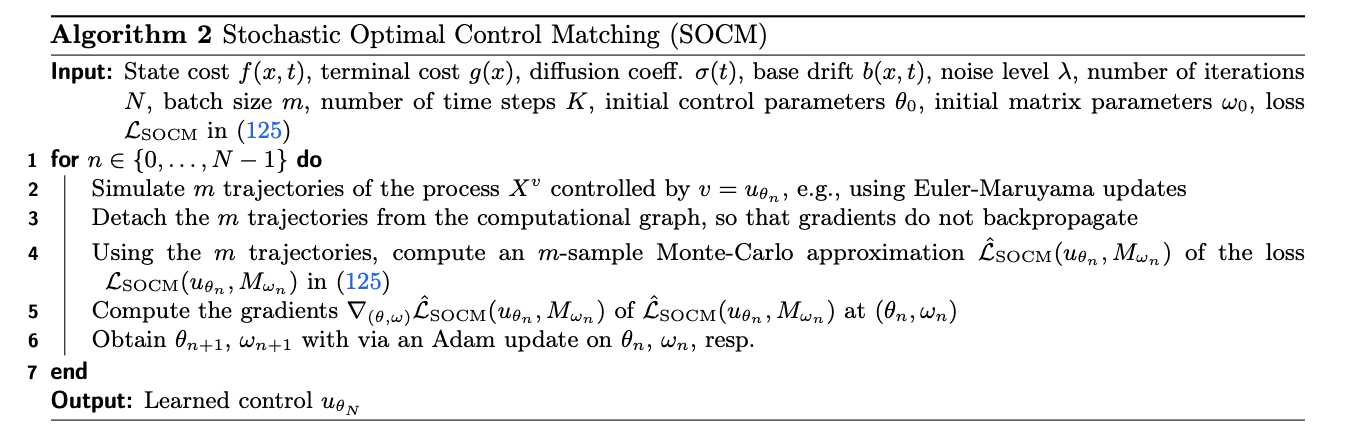
\includegraphics[width=0.95\textwidth]{figures/SOCM_algo.png}
        \caption{Stochastic Optimal Control Matching (SOCM) Algorithm}
    \end{figure}
\end{frame}

%------------------------------------------------

%------------------------------------------------

\section{Experiments and results}

\begin{frame}[allowframebreaks]{Ornstein-Uhlenbeck Process Benchmarks}
    \vspace{-0.3cm}
    
    \begin{block}{What's an Ornstein-Uhlenbeck (OU) Process?}
        A \textcolor{blue}{\textbf{mean-reverting}} stochastic differential equation with linear drift and Gaussian noise:
        $$dX_t = \theta(\mu - X_t) dt + \sigma dB_t \quad \text{(1D case)}$$

        The Ornstein-Uhlenbeck process is a classic mean-reverting SDE with both drift and noise, simple enough to solve analytically but rich enough to test stochastic control methods. It serves as the ideal benchmark for evaluating SOCM's bias-variance tradeoff
    \end{block}
    
    \vspace{0.8cm}
    
\end{frame}

\begin{frame}{Experimental Results (1/2)}
    \begin{figure}
        \centering
        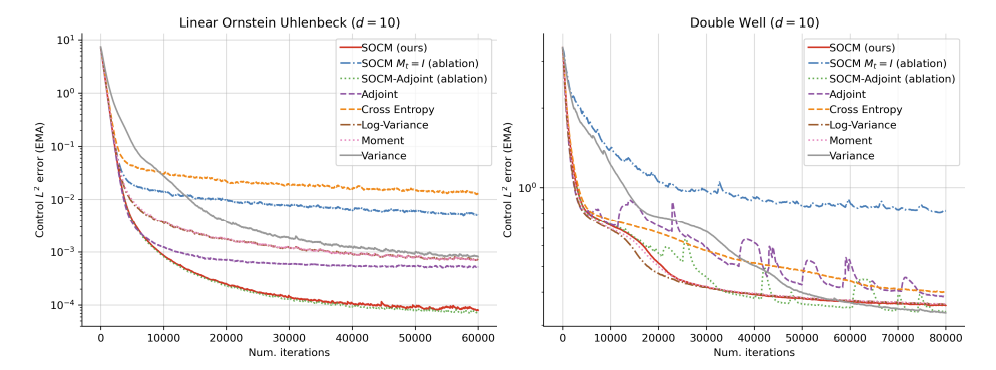
\includegraphics[width=0.95\textwidth]{figures/plots_1.png}
    \end{figure}
\end{frame}

\begin{frame}{Experimental Results (2/2)}
    \begin{figure}
        \centering
        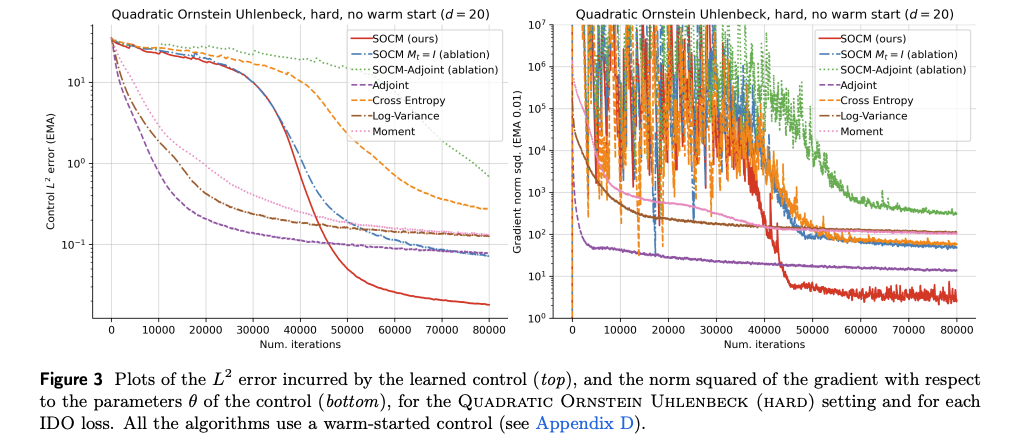
\includegraphics[width=0.95\textwidth]{figures/plots_2.png}
    \end{figure}
    % \note{At the end of training, SOCM obtains the lowest L2
    %     error, improving over all existing methods by a factor of
    %     around ten. The two SOCM ablations come in second and third by a substantial difference, which underlines
    %     the importance of the path-wise reparameterization trick.
    %     \\
    %     \textcolor{red}{JE DOIS COMPRENDRE CE QUE EST UN ORNSTEIN UHLENBECK PROCESS}
    %     }
\end{frame}

%------------------------------------------------

%------------------------------------------------
\section{Conclusion}

\begin{frame}{Conclusion}

    \begin{block}{Personal thoughts and conclusion}

    SOCM is a framework grounded in theory that has shown interesting empirical results in specific benchmarks, but to truly judge its potential further application of this framework needs to be explored. 
    \\
    \vspace{0.2cm}
    This said the authors seems to have already identified a few difficulties with this approach being the high variance related to the factor alpha(v, Xv, B) due to a mismatch between the probability measures induced by the learned control and the optimal control. This is a problem that is also encountered in out-of-distribution generalization for reinforcement learning.
    \\
    \vspace{0.2cm}
    Additionally, I would love to come back to this paper in the next year after having acquired a proper foundation in stochastic calculus, partial differential equations, and statistical mechanics.

    \end{block}

    \note{The main roadblock when we try to apply SOCM to more challenging problems is that the variance of the
        factor alpha(v, Xv, B) explodes when f and/or g are large, or when the dimension d is high. The control L2 error
        for the SOCM and cross-entropy losses remains high and fluctuates heavily due to the large variance of alpha
        The large variance of alpha is due to the mismatch between the probability measures induced by the learned
        control and the optimal control. Similar problems are encountered in out-of-distribution generalization for
        reinforcement learning, and some approaches may be carried over from that area (Munos et al., 2016).}
\end{frame}

%! so many links to do with RL and Monte Carlo Markov Chains which representent discretized differential equations
%------------------------------------------------

% \begin{frame}{Blocks of Highlighted Text}
%     In this slide, some important text will be \alert{highlighted} because it's important. Please, don't abuse it.

%     \begin{block}{Block}
%         Sample text
%     \end{block}

%     \begin{alertblock}{Alertblock}
%         Sample text in red box
%     \end{alertblock}

%     \begin{examples}
%         Sample text in green box. The title of the block is ``Examples".
%     \end{examples}
% \end{frame}


% \begin{frame}{References}
%     \footnotesize
%     \bibliography{reference.bib}
%     \bibliographystyle{apalike}
% \end{frame}

%------------------------------------------------

\end{document}